\documentclass{beamer}


\graphicspath{{figures/}}
\usepackage{tikz}
%\usetheme{boxes}
\usepackage[utf8]{inputenc}
\usepackage{amsmath}
\usepackage{amsthm}
\usepackage{hyperref}

\usepackage{booktabs}
\usepackage{natbib}
\bibliographystyle{abbrvnat}
\usecolortheme{crane}

\definecolor{orange}{RGB}{232, 86, 15}
\definecolor{blue}{RGB}{14, 159, 232}
\definecolor{blueblue}{RGB}{50, 90, 160}
\definecolor{yellow}{RGB}{232, 187, 14} 
\definecolor{red}{RGB}{232, 14, 59}

\hypersetup{
  colorlinks=true,
  linkcolor=cyan,
  urlcolor=cyan,
  citecolor=purple
}
\newtheorem{deff}{Definición}
%Information to be included in the title page:
\institute[]{}

\setbeamercolor{title}{bg=blueblue, fg=white}
\setbeamercolor{subttile}{bg=blueblue, fg=white}
\setbeamercolor{frametitle}{bg=blueblue, fg=white}
\setbeamercolor{block title}{bg=blue, fg=white}
\setbeamercolor{block title alerted}{bg=red, fg=white}
\setbeamercolor{block title example}{bg=yellow, fg=white}
\setbeamercolor{footline}{bg=gray, fg=white}

\beamertemplatenavigationsymbolsempty

\title{Gherardo Varando}
\author{Gherardo Varando}
\date{25 March 2025}
\begin{document}

\begin{frame}{(Casual) Causality Course 2025}

	\begin{block}{Intructors}
	  \begin{itemize}
	    \item Gherardo \url{gherardo.varando@uv.es}
	    \item Emiliano \url{emiliano.diaz@uv.es} 
	    \item Vassilis \url{vasileios.sitokonstantinou@uv.es}
	  \end{itemize}
	\end{block}
	
	\begin{block}{Schedule} 
         \begin{itemize}
	   \item \textbf{week 1, Tuesday} Intro and causal inference (GV)
	   \item \textbf{week 1, Thursday}     
	   \item \textbf{week 2, Tuesday} Causal Discovery (ED)
	   \item \textbf{week 2, Thursday} Causal Discovery (ED)
	   \item \textbf{week 3} Intensive weeek with group projects! 
	 \end{itemize}
	\end{block}


\end{frame}


\begin{frame}{Learning outcomes} 

  \begin{columns}
    \begin{column}{0.5\textwidth}
  \begin{itemize}[<+-|alert@+>]
    \item Understand the fundamental
          goals and problems of causal methods  
    \item Familiarize with the vocabulary, definitions and basic concepts of causality
    \item Understand the fundamentals behind basic methodologies in
          causal inference and causal discovery
	\item How causal methods and tools are relevant in ML?
  \end{itemize}
    \end{column}
    \begin{column}{0.5\textwidth}
      \only<1>{
	\begin{figure}
	  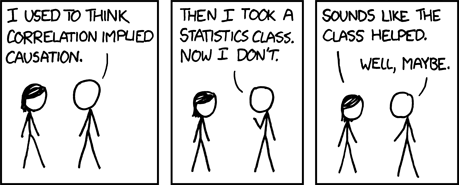
\includegraphics[width=5cm]{correlation}
	  \caption{xkcd (CC BY-NC 2.5) \url{https://xkcd.com/552}}
	\end{figure}
      }
\only<2>{
	\begin{figure}
	  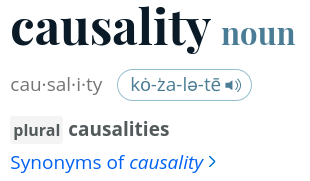
\includegraphics[width=5cm]{causality_noun}
	  \caption{\url{https://www.merriam-webster.com/dictionary/causality}}
	\end{figure}
      }
\only<3>{
	\begin{figure}
	  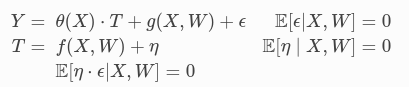
\includegraphics[width=5cm]{dml}
	  \caption{\url{https://econml.azurewebsites.net}}
	\end{figure}
      }
 \only<4>{
	\begin{figure}
	  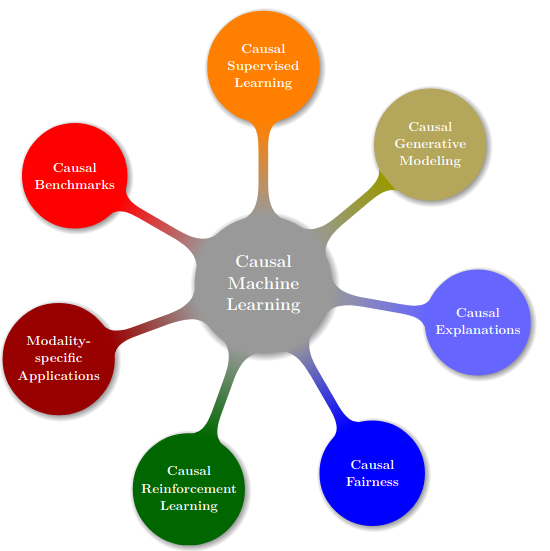
\includegraphics[width=5cm]{causal_ml}
	  \caption{From \cite{kaddour2022causalmachinelearningsurvey}}
	\end{figure}
      }
    \end{column}
  \end{columns}
\end{frame}

\begin{frame}{Content week 1}
  \begin{itemize}
    \item \textbf{Session 1} Tue 25/03
      \begin{itemize}
	\item[Part I] Intro to causality and causal methods
	\item[Part II] Basics of causal inference
      \end{itemize}
    \item \textbf{Session 2} Thu 27/03
      \begin{itemize}
	\item[Part I] Causal inference methods
	\item[Part II] Robustness to interventions  
      \end{itemize}
  \end{itemize}
\end{frame}

\begin{frame}{Basic references}
  \begin{itemize}
    \item \href{https://mitpress.mit.edu/9780262037310/elements-of-causal-inference/}{Elements of causal inference} \citep{peters2017elements} 
    \item \href{https://miguelhernan.org/whatifbook}{Causal Inference: What If} \citep{hernan2025causal}
    \item All of Statistics \citep{wasserman2013all} 
  \end{itemize}
  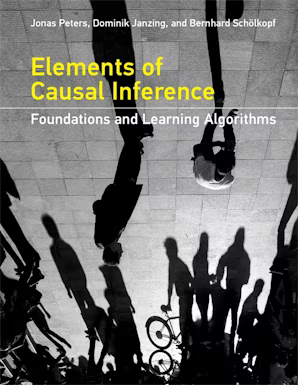
\includegraphics[width = 2 cm]{elements}
  
\includegraphics[width = 2 cm]{whatif}
  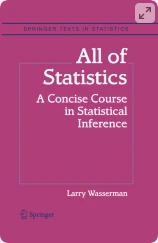
\includegraphics[width = 2 cm]{all}
\end{frame}


\begin{frame}{What is causality?}
  \begin{center}
    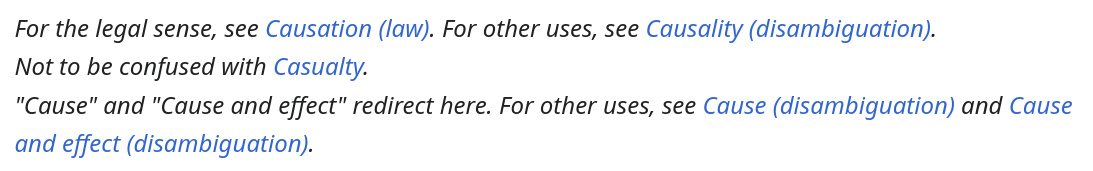
\includegraphics[width=0.95\textwidth]{Causality-Wikipedia}
  \end{center}
  \begin{itemize}
    \item Causality in Law  \url{https://en.wikipedia.org/wiki/Causation_(law)}
      \href{https://www.youtube.com/watch?v=XiCOmhdkM80&list=PLqMxKp2ot-3vDaLyaAZNgt8ijj6n0l460}{Causation|Low of Tort playlist on youtube, first 3 videos}  
    \item Causality in Physics \\
       \url{https://en.wikipedia.org/wiki/Causality_(physics)}  \\
       \url{https://www.youtube.com/watch?v=eG_eHDDMgCs} \\
       \cite{rovelli2022causationrootedthermodynamics}  
  \end{itemize}
\end{frame}
 
\begin{frame}{On the concept of \emph{Harm}} 
  \begin{itemize}
    \item \cite{sarvet2023perspective}  interventionalist vs contrefactual  
    \item \cite{mueller2024perspective} response 
  \end{itemize}
\end{frame}


\begin{frame}{Personalized decision making}
  \begin{itemize}
    \item \cite{mueller2023personalized} 
    \item \cite{tian2000probabilities} 
  \end{itemize}
\end{frame}


\begin{frame}[allowframebreaks]{Bibliography}
\bibliography{biblio}
\end{frame}

\end{document}


